% ClapCap -- ISMIR-style two-column paper.
% Build: pdflatex main && pdflatex main (manual thebibliography, no bibtex).
\documentclass{article}
\usepackage[T1]{fontenc}
\usepackage[utf8]{inputenc}
\usepackage{ismir,amsmath,url}
\usepackage{graphicx}
\usepackage{amssymb}
\usepackage{booktabs}
\usepackage{tabularx}
\usepackage{placeins}
\usepackage{tikz}
\usepackage{xcolor}
\usepackage[colorlinks=true,citecolor=red,urlcolor=black,bookmarks=false,pagebackref=true]{hyperref}
\hypersetup{linkcolor=green!45!black}
\renewcommand{\permission}{}  % suppress the proceedings attribution block

% headings render as typed: \uppercase removed in ismir.sty (title, \@sect, abstract)
\usetikzlibrary{arrows.meta,positioning,fit,backgrounds}

\newcommand{\fense}{\textsc{Fense}}
\newcommand{\clapenc}{\textsc{Clap}}
\newcommand{\sys}{\textsc{ClapCap}}

% Title in IEEE-compliant title case.
\title{ClapCap: Lightweight Prefix-Conditioned Language Models for Music Captioning via a CLAP-to-LM Architecture}

\oneauthor{Ali Ozkaya}{Department of Computer Engineering \\ Izmir Institute of Technology}
\def\authorname{A. Ozkaya}

\sloppy

\begin{document}
\maketitle
\pagestyle{plain}\thispagestyle{plain}  % page numbers (remove for camera-ready)

\begin{abstract}
We study whether a \emph{lightweight} language model (LM) can describe music when fed
nothing but a short, learned prefix projected from a frozen audio embedding. Our pipeline,
\sys{}, is the audio analogue of ClipCap~\cite{mokady2021clipcap}: a frozen \clapenc{} audio
encoder produces a single clip embedding, a small projection network maps it to a fixed-length
prefix of pseudo-tokens, and a pretrained LM autoregressively generates the caption. On
MusicCaps~\cite{agostinelli2023musiclm} we run a controlled comparison of two LM families ---
GPT-2 (decoder-only, 124M) and T5-base (encoder--decoder, 220M) --- holding the encoder,
projection, data split and evaluation fixed so that the LM is the only variable. We report a
ten-metric suite with \fense{}~\cite{zhou2022fense} as the primary score, and we measure a
per-model \emph{noise floor} from three seeds so that every ablation delta can be judged against
run-to-run variance. We find that (i) the two LMs are statistically indistinguishable at
baseline once the noise floor is accounted for; (ii) second-stage fine-tuning erases nearly all
architectural differences introduced in the projection stage; (iii) the largest decoding lever,
sentence completion, improves \fense{} mostly by removing the fluency-error term rather than by
improving semantics; and (iv) the models capture genre, instrumentation and mood
well but share a systematic male-vocalist bias, which we trace to caption-prior amplification
under uncertain audio evidence rather than to a missing audio cue. We frame the work as an
efficiency- and analysis-oriented study of the minimum viable architecture for music captioning,
not a state-of-the-art claim. Code is available at
\href{https://github.com/raccoon-42/audio-caption}{\texttt{github.com/raccoon-42/audio-caption}}.
\end{abstract}

\section{Introduction}\label{sec:intro}

Most audio captioning research targets \emph{general} sound --- environmental events and
acoustic scenes --- on AudioCaps~\cite{kim2019audiocaps} and Clotho~\cite{drossos2020clotho}.
Music is different: a useful music caption describes \emph{musical} attributes such as genre,
instrumentation, mood, tempo and structure rather than discrete sound events. This paper asks a
deliberately minimal question: \emph{can a lightweight language model understand music semantics
through a simple projection from a frozen audio embedding?}

Our approach, \sys{}, adapts ClipCap~\cite{mokady2021clipcap}, which captions images by
projecting a frozen CLIP embedding into a prefix of pseudo-tokens for GPT-2. We replace the image
encoder with a frozen \clapenc{} audio encoder~\cite{wu2023clap}, caption music instead of
images, and --- crucially --- turn the single-LM recipe into a \emph{controlled comparison} of
language models. Because the encoder, projection, data split and evaluation are all shared, the
language model is the only thing that changes between conditions.

The contributions of this paper are:
\begin{itemize}\itemsep2pt
  \item An audio adaptation of the ClipCap prefix-captioning recipe to music, with a single
        shared evaluation harness.
  \item A \emph{noise-floor} methodology: per-model run-to-run variance from three seeds, so
        single-run ablation deltas are interpretable rather than anecdotal.
  \item A controlled comparison of a decoder-only (GPT-2) and an encoder--decoder (T5) LM, with
        ablations over projection architecture and decoding strategy.
  \item A qualitative and statistical analysis of a recurring vocalist bias, which we trace to
        caption-prior amplification under uncertain audio evidence rather than to the audio
        frontend alone.
\end{itemize}

This paper does not claim state-of-the-art performance. Published captioning systems are
evaluated on different datasets with different reference counts, so a numerical comparison
would be meaningless (Section~\ref{sec:related}), and we do not attempt one. The contribution
is the controlled analysis itself, together with the efficiency of the recipe --- only a small
projection (plus the LM) is trained.

\section{Related Work}\label{sec:related}

\textbf{Prefix captioning.}
ClipCap~\cite{mokady2021clipcap} maps a frozen CLIP image embedding to a constant-length prefix
($K{=}10$ tokens) consumed by GPT-2, training only a small mapping network. It offers two design
points: a lightweight transformer mapper with a frozen LM, and an MLP mapper with a fine-tuned
LM. \sys{} is the audio analogue of the MLP-mapper, fine-tuned-LM variant. Notably, ClipCap
reports that this variant \emph{overfits} as trainable capacity grows --- an observation we
recover, amplified, when scaling the LM (Section~\ref{sec:limitations}). In the audio domain,
Pengi~\cite{deshmukh2023pengi} likewise conditions a small LM on an audio-derived prefix,
framing a range of audio tasks as text generation.

\textbf{General audio captioning.}
Audio captioning is typically benchmarked on AudioCaps~\cite{kim2019audiocaps} and
Clotho~\cite{drossos2020clotho}, which describe general sounds and provide multiple references
per clip. These differ from music captioning in domain, number of references, and the metrics
commonly reported (CIDEr/SPIDEr rather than the semantic \fense{}). Cross-dataset numerical
comparison is therefore not meaningful, and we avoid it.

\textbf{Music captioning.}
MusicCaps~\cite{agostinelli2023musiclm} is a hand-curated set of 5{,}521 ten-second clips from
AudioSet~\cite{gemmeke2017audioset}, each annotated by musicians with a multi-sentence caption and a list of musical
aspects. LP-MusicCaps~\cite{doh2023lpmusiccaps} addresses caption scarcity by generating
pseudo-captions with an LLM over tag datasets and trains a convolutional-encoder/BART-decoder
captioner. Such domain-specific captioners are a natural \emph{reference} for \sys{}, but a fair
comparison must run them on our exact test split and avoid the leakage that arises when a
captioner is itself trained on MusicCaps; we leave this to future work.

\textbf{Audio language models.}
End-to-end audio LLMs such as Qwen-Audio~\cite{chu2023qwenaudio} and
SALMONN~\cite{tang2024salmonn} couple a large LM to an audio encoder and are trained on large
instruction corpora. They are far heavier than the present recipe; we regard them as an
upper-bound reference direction rather than a controlled comparison, since they bypass the
frozen-encoder/learned-prefix design we study.

\section{Method}\label{sec:method}

\textbf{Overview.}
A clip is encoded once by a frozen \clapenc{} model into a $d_a$-dimensional embedding. A
projection network $f_\theta$ maps this vector to a prefix
$p_1,\dots,p_k \in \mathbb{R}^{d_{\text{lm}}}$ of $k$ pseudo-tokens in the LM embedding space.
The LM then generates the caption autoregressively, conditioned on the prefix
(Figure~\ref{fig:pipeline}).

\begin{figure*}[t]\centering
\footnotesize
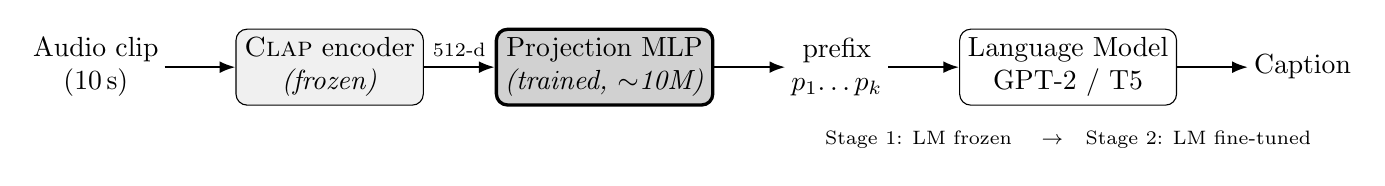
\begin{tikzpicture}[
    node distance=6mm and 9mm,
    box/.style={draw, rounded corners, minimum height=9mm, align=center, inner sep=3pt},
    frozen/.style={box, fill=black!6},
    trained/.style={box, fill=black!18, very thick},
    data/.style={align=center, inner sep=2pt},
    flow/.style={-{Latex[length=2mm]}, thick}]
  \node[data] (audio) {Audio clip\\(10\,s)};
  \node[frozen, right=of audio] (clap) {\clapenc{} encoder\\\emph{(frozen)}};
  \node[trained, right=of clap] (proj) {Projection MLP\\\emph{(trained, $\sim$10M)}};
  \node[data, right=of proj] (prefix) {prefix\\$p_1\!\dots p_k$};
  \node[box, right=of prefix] (lm) {Language Model\\GPT-2 / T5};
  \node[data, right=of lm] (cap) {Caption};
  \draw[flow] (audio) -- (clap);
  \draw[flow] (clap) -- node[above,font=\scriptsize]{512-d} (proj);
  \draw[flow] (proj) -- (prefix);
  \draw[flow] (prefix) -- (lm);
  \draw[flow] (lm) -- (cap);
  \node[font=\scriptsize, below=2mm of lm, align=center] (s) {Stage~1: LM frozen \quad$\rightarrow$\quad Stage~2: LM fine-tuned};
\end{tikzpicture}
\caption{The \sys{} pipeline. A frozen \clapenc{} encoder turns the audio clip into a single
512-d embedding; a small projection MLP (the only newly added module) maps it to a $k$-token
prefix in the LM embedding space; the LM generates the caption. Stage~1 trains the projection
with the LM frozen; Stage~2 additionally fine-tunes the LM.}
\label{fig:pipeline}
\end{figure*}

\textbf{Audio encoder.}
We use the LAION \clapenc{} checkpoint \texttt{laion/clap-htsat-unfused}~\cite{wu2023clap},
whose audio tower is an HTS-AT transformer~\cite{chen2022htsat} producing a $512$-dimensional
audio embedding. \clapenc{} is trained on general audio and is \emph{not}
music-specialised --- a deliberate test of how far a general frontend carries on a music task,
and a limitation we revisit. Embeddings are precomputed once and cached, so the encoder never
runs during training or evaluation. The ``unfused'' variant ingests a fixed $\sim$10\,s window,
matching MusicCaps clip length.

\textbf{Projection network.}
The projection is a small MLP,
$\text{Linear}\!\rightarrow\!\text{LayerNorm}\!\rightarrow\!\text{GELU}\!\rightarrow\!
\text{Dropout}\!\rightarrow\!\text{Linear}$, reshaped to $(k,d_{\text{lm}})$. The baseline uses
prefix length $k{=}8$, dropout $0.3$ and depth $2$.

\textbf{Language models.}
We compare GPT-2~\cite{radford2019gpt2} (decoder-only, 124M) and T5-base~\cite{raffel2020t5}
(encoder--decoder, 220M). For T5 the prefix is fed to the encoder; for GPT-2 it is prepended as
input embeddings. Extending the same harness to modern billion-parameter decoders is in progress
(Section~\ref{sec:limitations}).

\textbf{Two-stage training.}
In Stage~1 (S1) the LM is frozen and only the projection is trained; in Stage~2 (S2) the
projection and the full LM are fine-tuned together (the audio encoder stays frozen). S1
corresponds to ClipCap's frozen-LM regime and S2 to its fine-tuned-LM regime. The objective in
both stages is autoregressive cross-entropy on caption tokens conditioned on the prefix,
\[
  \mathcal{L} = -\sum_{j}\log p_\theta\!\left(c_j \mid p_1,\dots,p_k, c_1,\dots,c_{j-1}\right).
\]
We use AdamW~\cite{loshchilov2019adamw} (weight decay $0.1$), cosine
annealing~\cite{loshchilov2017sgdr}, batch size $8$ and early stopping
(patience $5$). Per model, only the learning rates are tuned, via a 16-trial
Optuna~\cite{akiba2019optuna} search over an 8-epoch proxy; all else is fixed so the LM stays
the controlled variable.

\textbf{Efficiency.}
The only newly added module is the projection ($\sim$$10.2$M parameters): Stage~1 trains it
alone with the LM frozen, and Stage~2 additionally fine-tunes the LM. The complete model is
$124$M (GPT-2) or $220$M (T5) parameters --- one to two orders of magnitude smaller than the
billion-parameter end-to-end audio LLMs --- and every experiment in this paper runs on a
single consumer GPU (NVIDIA RTX~5090). Because \clapenc{} embeddings are precomputed once,
the audio encoder is never run during training.

\section{Experimental Setup}\label{sec:setup}

\textbf{Data.}
We use MusicCaps~\cite{agostinelli2023musiclm} with a fixed three-way random split: a held-out
test set ($n{=}529$, final metrics only), a validation set ($n{\approx}495$, for checkpoint
selection and hyperparameter search), and the remainder for training ($n{\approx}4{,}455$). The
split seed is fixed across all conditions, so every model and seed is scored on the identical
test set.

\textbf{Metrics.}
A single shared harness scores all conditions with the \texttt{aac-metrics} suite: BLEU-1 and
BLEU-4~\cite{papineni2002bleu}, METEOR~\cite{banerjee2005meteor}, ROUGE-L~\cite{lin2004rouge},
CIDEr-D~\cite{vedantam2015cider}, SPICE~\cite{anderson2016spice}, SPIDEr~\cite{liu2017spider},
SBERT-sim, FER and \fense{}.
\fense{}~\cite{zhou2022fense} is our primary metric: it combines a
Sentence-BERT~\cite{reimers2019sbert} semantic similarity with a fluency-error penalty (FER),
making it sensitive to the semantic correctness a listener cares about. We apply no post-processing by default; sentence trimming is treated as an
explicit decoding ablation (Section~\ref{sec:decoding}).

\textbf{Noise floor.}
To judge whether a delta is real, we retrain each baseline with three seeds (42,\,43,\,44),
varying only initialisation, shuffling and dropout while holding the data split fixed. The
standard deviation of each metric across seeds is our \emph{noise floor}; deltas smaller than it
are not interpreted as effects.

\section{Results}\label{sec:results}

\subsection{Baseline comparison}\label{sec:baseline}
Table~\ref{tab:baseline} reports greedy-decoding test metrics with per-model noise floors. GPT-2
leads on every metric, including the primary \fense{} ($0.3998$ vs.\ $0.3954$), but the margin
($0.004$) is smaller than either model's \fense{} noise floor ($\pm0.0137$ for GPT-2,
$\pm0.0345$ for T5). We therefore do \emph{not} read it as evidence that one architecture is
better at music captioning under this recipe. The noise floor is also $\sim$$2.5\times$ larger
for T5 than GPT-2, so the encoder--decoder is noticeably noisier run-to-run and each model must
be judged against its \emph{own} variance.

\begin{table*}[t]
\centering
\caption{Baseline (greedy) test-set metrics for both language models, with per-model run-to-run standard deviation (noise floor) from three seeds. \textsc{Fense} is the primary metric; best per column in bold.}
\label{tab:baseline}
\footnotesize
\setlength{\tabcolsep}{4pt}
\begin{tabular}{lrrrrrrrrrr}
\toprule
Model & BLEU-1 & BLEU-4 & METEOR & ROUGE-L & CIDEr-D & SPICE & SPIDEr & SBERT-sim & FER & FENSE \\
\midrule
GPT-2 & \textbf{0.3091} & \textbf{0.0631} & \textbf{0.1265} & \textbf{0.2329} & \textbf{0.1109} & \textbf{0.1091} & \textbf{0.1100} & \textbf{0.5820} & \textbf{0.3478} & \textbf{0.3998 {\scriptsize$\pm$0.0137}} \\
T5 & 0.3003 & 0.0574 & 0.1162 & 0.2275 & 0.0847 & 0.0866 & 0.0857 & 0.5564 & 0.3251 & 0.3954 {\scriptsize$\pm$0.0345} \\
\bottomrule
\end{tabular}
\\[2pt]{\footnotesize\emph{The GPT-2/T5 \textsc{Fense} gap (0.004) is smaller than either model's noise floor, i.e. not significant.}}
\end{table*}


\FloatBarrier
\subsection{Stage~1 vs.\ Stage~2}\label{sec:stages}
Figure~\ref{fig:training} shows validation loss per epoch for every projection configuration.
In Stage~1, where only the projection is trained, the configurations spread widely (a range of
$0.38$ for GPT-2 and $0.83$ for T5). After Stage~2 fine-tuning that spread collapses to $0.03$
for both models: full fine-tuning largely erases the architectural differences introduced by the
projection. The S2 curves also reveal early overfitting --- validation loss bottoms within a few
epochs and then rises --- which early stopping handles.

\begin{figure*}[t]\centering
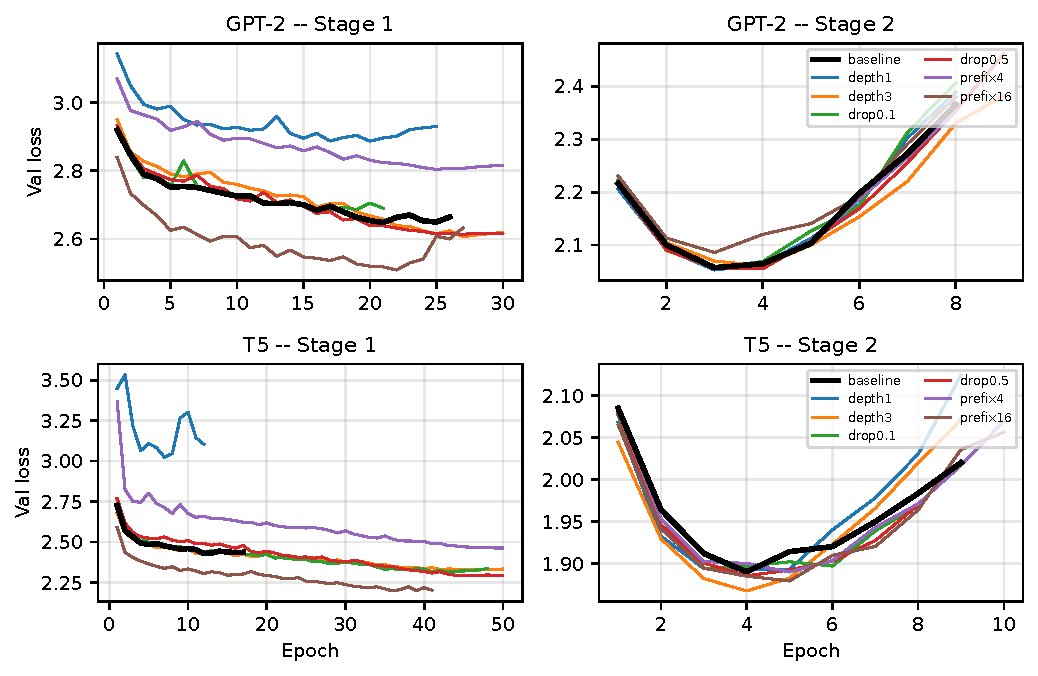
\includegraphics[width=\textwidth]{figures/fig_training_curves.pdf}
\caption{Validation loss per epoch for all projection configurations. \emph{Left:} Stage~1
(projection only) shows a wide spread across configurations. \emph{Right:} Stage~2 (full
fine-tuning) collapses that spread --- the configurations become nearly indistinguishable ---
and shows the early-overfitting onset. The baseline is drawn in bold.}
\label{fig:training}
\end{figure*}

\FloatBarrier
\subsection{Architecture ablations}\label{sec:arch}
We vary prefix length ($\{4,16\}$ around $8$), dropout ($\{0.1,0.5\}$ around $0.3$) and
projection depth ($\{1,3\}$ around $2$), retraining each from scratch with greedy decoding.
Figure~\ref{fig:arch} plots the resulting \fense{} against the baseline $\pm$ noise-floor band.
Consistent with Section~\ref{sec:stages}, most configurations fall within the band: no projection
hyperparameter reliably moves the primary metric for GPT-2. For T5 the prefix variants produce
larger \fense{} swings, but --- as the next section shows --- these coincide with collapses in
the fluency-error term rather than genuine semantic gains.

\begin{figure*}[t]\centering
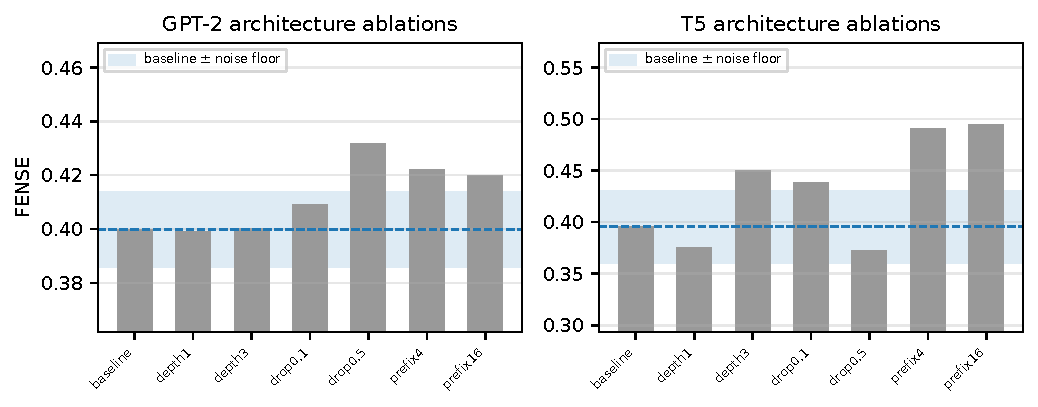
\includegraphics[width=\textwidth]{figures/fig_arch_noisefloor.pdf}
\caption{Architecture-ablation \fense{} per configuration. The shaded band is the baseline
$\pm$ one noise-floor standard deviation. Bars inside the band are not distinguishable from the
baseline.}
\label{fig:arch}
\end{figure*}

\FloatBarrier
\subsection{Decoding ablations}\label{sec:decoding}
Decoding strategies are evaluated on the fixed baseline checkpoint (no retraining), isolating
generation behaviour. Table~\ref{tab:decoding} lists the top configurations by \fense{}. The
dominant lever is trimming trailing incomplete sentences: it lifts \fense{} from $0.3998$ to
$0.5796$ for GPT-2 and from $0.3954$ to $0.5762$ for T5.

This gain is, however, \emph{largely an artifact of the metric}. Figure~\ref{fig:fensefer} plots
\fense{} against FER across all decoding configurations: the relationship is almost perfectly
inverse, and the trimmed configurations simply drive FER to near zero while the lexical metrics
in Table~\ref{tab:decoding} barely move. In other words, trimming removes the
fluency penalty inside \fense{} without making captions semantically more correct. We report it
as a useful decoding choice for producing clean captions, but caution against reading the
headline \fense{} jump as a semantic improvement.

\begin{figure*}[t]\centering
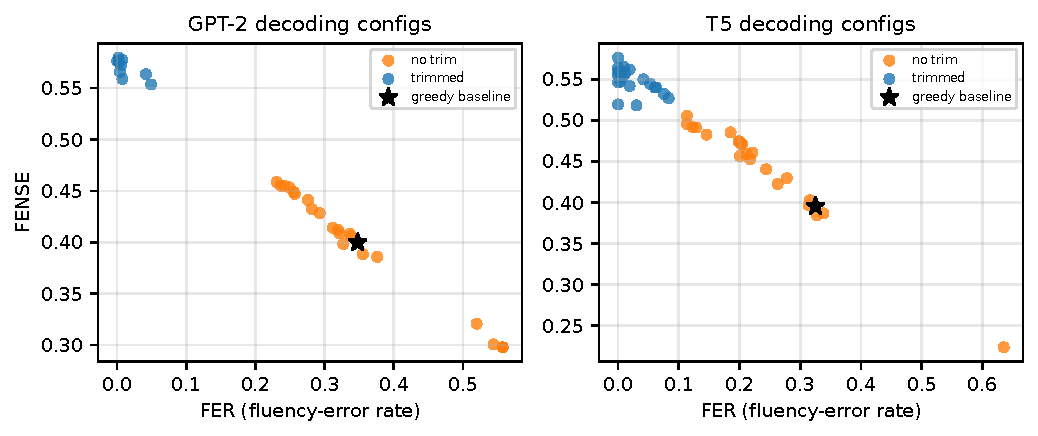
\includegraphics[width=\textwidth]{figures/fig_decoding_fense_fer.pdf}
\caption{\fense{} vs.\ FER over all decoding configurations. The near-perfect inverse trend shows
that \fense{} here is dominated by the fluency-error term: trimmed configurations (low FER) score
high \fense{} without improving semantic similarity. The star is greedy decoding.}
\label{fig:fensefer}
\end{figure*}

\begin{table*}[t]
\centering
\caption{Top decoding configurations per model (eval-only on the baseline checkpoint), ranked by \textsc{Fense}. Note that high \textsc{Fense} coincides with near-zero FER while lexical metrics (CIDEr-D, SPIDEr) barely move -- see Figure~\ref{fig:fensefer}.}
\label{tab:decoding}
\footnotesize
\setlength{\tabcolsep}{4pt}
\begin{tabular}{lrrrrr}
\toprule
Config & FENSE & SBERT-sim & FER & CIDEr-D & SPIDEr \\
\midrule
\multicolumn{6}{l}{\textbf{GPT-2}} \\
greedy (baseline) & 0.3998 & 0.5820 & 0.3478 & 0.1109 & 0.1100 \\
trim\_ngram2 & \textbf{0.5796} & 0.5807 & 0.0019 & 0.1092 & 0.1087 \\
trim\_rep1.2\_ngram2\_t0.3 & 0.5775 & 0.5812 & 0.0076 & 0.1003 & 0.1033 \\
trim\_rep1.2\_ngram2 & 0.5766 & 0.5766 & 0.0000 & 0.0959 & 0.1000 \\
trim\_rep1.2\_ngram3 & 0.5766 & 0.5781 & 0.0019 & 0.0926 & 0.0986 \\
trim\_rep1.2 & 0.5758 & 0.5774 & 0.0019 & 0.0924 & 0.0983 \\
trim\_rep1.3 & 0.5723 & 0.5748 & 0.0057 & 0.0885 & 0.0938 \\
\midrule
\multicolumn{6}{l}{\textbf{T5}} \\
greedy (baseline) & 0.3954 & 0.5564 & 0.3251 & 0.0847 & 0.0857 \\
trim\_rep1.2 & \textbf{0.5762} & 0.5762 & 0.0000 & 0.0863 & 0.0892 \\
trim\_beam5\_ngram2 & 0.5649 & 0.5698 & 0.0095 & 0.0878 & 0.0945 \\
trim\_rep1.3 & 0.5640 & 0.5640 & 0.0000 & 0.0779 & 0.0883 \\
trim\_rep1.2\_beam5\_ngram2 & 0.5618 & 0.5716 & 0.0189 & 0.0985 & 0.1004 \\
trim\_rep1.2\_ngram2 & 0.5593 & 0.5593 & 0.0000 & 0.0662 & 0.0831 \\
trim\_rep1.2\_ngram2\_t0.3 & 0.5591 & 0.5599 & 0.0019 & 0.0611 & 0.0792 \\
\bottomrule
\end{tabular}
\end{table*}


\FloatBarrier
\subsection{Qualitative analysis}\label{sec:qual}
Table~\ref{tab:qual} shows representative successes and failures. The models reliably recover
high-level musical content --- genre (rock, jazz, electronic), instrumentation (electric guitar,
bass, drums, piano) and mood (groovy, energetic, emotional). Two failure modes recur: on
\emph{non-music} audio the pipeline still emits a confident music caption, and greedy decoding
occasionally degenerates into verbatim repetition. Most strikingly, both models tend to insert ``a male
vocalist singing melodically'' even when the reference explicitly states there is no singer.

To characterise this we measured vocal-presence and vocalist-gender agreement over the full
test set. The bias is \emph{not} a blind spot: GPT-2 mentions vocals on 95\% of clips whose
reference describes singing, but also on 43\% of clips marked instrumental (T5: 82\%\,/\,29\%)
--- both models track vocal presence well above chance while skewing toward false positives.
The skew mirrors the training captions, of which 53\% mention vocals and in which male
vocalists outnumber female ones 2.2:1; the phrase ``male vocalist'' appears in 10\% of training
captions but in roughly half of the generated ones. Gender is worse: on references describing a
\emph{female} singer, T5 outputs ``male'' 89\% of the time and GPT-2 44\%, while male
references are almost never misgendered (2--4\%). These rates persist across decoding
configurations, so they are not a decoding artifact.

To separate the frontend from the LM, we probed the frozen \clapenc{} embeddings directly with
zero-shot text prompts: vocal vs.\ instrumental is separable at 74\% accuracy and vocalist
gender at 76\% (female recall only 55\%). The embedding therefore carries the relevant cues,
but noisily --- and since both LMs read the \emph{same} embedding, the gap between GPT-2
(56\%) and T5 (11\%) in female-vocalist accuracy shows the failure is largely model-side. We
conclude that the vocalist bias is caption-prior amplification under uncertain audio evidence,
not a missing audio cue: a music-specialised encoder should sharpen the evidence, but the
male-vocalist default itself is learned from the caption statistics.

\begin{table*}[t]
\centering
\footnotesize
\caption{Representative successes and failures (baseline greedy; captions trimmed at the last full sentence for display). The models recover genre, instrumentation and mood, but default to a male vocalist even on instrumental or non-music audio.}
\label{tab:qual}
\begin{tabularx}{\textwidth}{lX}
\toprule
\multicolumn{2}{c}{\textbf{Successes}}\\
\midrule
\addlinespace[2pt]
\emph{Reference} & instrumental rock music with a drum kit, lots of cymbal crashes, acoustic guitar strumming, harmonized lead guitars and an active bass guitar. \\
\emph{GPT-2} & This is a rock music piece. There is a male vocalist singing melodically. The electric guitar is playing the main tune while the bass guitar is playing in the background. The rhythmic background consists of a simple acoustic drum beat. The atmosphere is groovy. \\
\emph{T5} & This is a rock music piece. There is a male vocalist singing melodically. The electric guitar is playing a simple tune with a bass guitar playing in the background. The rhythmic background consists of a fast-paced acoustic drum beat. \\
\midrule
\addlinespace[2pt]
\emph{Reference} & This is a drum \& bass electronic music piece. There is no singer. There is a strong and fuzzy feeling bass sound. The rhythmic background consists of a loud and high tempo electronic drum beat. The atmosphere is modern and energetic. This piece could be playing at a nightclub or a dance club. \\
\emph{GPT-2} & This is a techno music piece. There is a male vocalist singing melodically. The melody is being played by the synth bass. The rhythmic background consists of a fast-paced electronic drum beat. The atmosphere is groovy. This piece could be used in the background of nightclubs. \\
\emph{T5} & This is a techno house music piece. There is a male vocalist singing melodically. The melody is being played by the synth bass while the rhythmic background consists of a fast-paced electronic drum beat. The atmosphere is energetic. \\
\midrule
\addlinespace[2pt]
\emph{Reference} & A female vocalist sings this melancholic melody in a foreign language. The tempo is slow with a romantic piano accompaniment. The song is soft, mellow, poignant, emotional, sentimental, romantic, melancholic, sad, lonely, and wistful. This song is a Pop/ Love song. \\
\emph{GPT-2} & This is a lullaby piece. There is a female vocalist singing melodically. The piano is playing a simple tune while the bass guitar is playing in the background. The atmosphere is calming and relaxing. This piece could be used in the background of a meditation video. \\
\emph{T5} & This is a classical music piece. There is a female vocalist singing melodically. The melody is being played by the piano while the rhythm is being played by the acoustic guitar. The atmosphere is romantic. \\
\midrule
\addlinespace[2pt]
\emph{Reference} & The low quality recording features a live performance of a jazz song and it consists of a groovy bass guitar, groovy rhodes keys, electric guitar melody, shimmering hi hats, punchy kick and punchy snare hits. It sounds groovy, funky and passionate. The recording is noisy and in mono. \\
\emph{GPT-2} & This is a jazz music piece. There is a saxophone solo being played. The melody is being played by the piano and the electric guitar. The rhythmic background consists of a simple acoustic drum beat. The atmosphere is groovy. This piece could be used in the background of a jazz bar. \\
\emph{T5} & This is a live recording of a jazz music piece. There is a saxophone playing the lead melody while a bass guitar is playing in the background. The rhythm is being played by the acoustic drums. The atmosphere is jazzy. \\
\midrule
\multicolumn{2}{c}{\textbf{Failure cases}}\\
\midrule
\addlinespace[2pt]
\emph{Reference} & The low quality recording features a printer that produces printing sounds and some muffled music playing in the background, probably on a radio. It is noisy and in mono. \\
\emph{GPT-2} & This is a recording of a live performance of a pop music piece. There is a male vocalist singing melodically. The melody is being played by a keyboard and a bass guitar while the rhythmic background is provided by a fast tempo electronic drum beat. \\
\emph{T5} & This is a live recording of a DJ performance. The DJ is scratching the turntable repeatedly. The turntable is a low quality recording. The sound of the turntable is distorted and the recording is of very poor quality. \\
\midrule
\addlinespace[2pt]
\emph{Reference} & The low quality recording features a metallic hit, followed by resonating bowl tone. The recording is mono and noisy. \\
\emph{GPT-2} & This is a meditation music piece. There is a bowl-like sound being played by the bowl. The bowl is being rubbed repeatedly. There is a calming and relaxing atmosphere to this piece. This piece can be used in the background of meditation videos. It can also be used in the background of meditation videos. \\
\emph{T5} & This is a Tibetan singing bowl playing in the background of a meditation video. There is a chanting bowl being played. There is a chanting bowl being played. There is a chanting bowl being played. There is a chanting bowl being played. \\
\bottomrule
\end{tabularx}
\end{table*}


\FloatBarrier
\section{Limitations and Future Work}\label{sec:limitations}

\textbf{General-purpose audio frontend.} Our encoder is trained on general audio, not music. A
music-specialised encoder (a music \clapenc{} checkpoint, MERT~\cite{li2024mert} or
MusicFM~\cite{won2024musicfm}) is a natural and likely beneficial swap, especially for the
fine-grained attributes (vocalist gender, instrument identity) where the embedding's cues are
noisiest (Section~\ref{sec:qual}).

\textbf{Capacity vs.\ data.} Scaling the LM is not free in this low-data regime
($\sim$4.5k clips). In preliminary runs a billion-parameter decoder fine-tuned end-to-end
overfits within a single epoch --- the same MLP-plus-fine-tuning overfitting that
ClipCap~\cite{mokady2021clipcap} reports, amplified by scale --- and requires a gentler schedule
to remain comparable. This supports the lightweight framing and motivates our in-progress
extension to such models.

\textbf{Metric caveats.} MusicCaps provides a single reference per clip, which mechanically
depresses n-gram metrics relative to multi-reference benchmarks. And as
Section~\ref{sec:decoding} shows, \fense{} can be inflated by fluency-driven trimming; we
mitigate this by reporting FER and lexical metrics alongside it.

\textbf{Reference and human evaluation.} We do not yet compare against a domain-specific music
captioner on our split; the clean route is a leakage-free checkpoint evaluated on our exact test
items via the same harness. We also plan an LLM-as-judge and human evaluation of semantic
correctness, reporting inter-rater agreement.

\section{Conclusion}\label{sec:conclusion}
We presented \sys{}, a controlled study of lightweight language models for \emph{music}
captioning via an audio adaptation of the ClipCap prefix recipe. Holding the frozen \clapenc{}
encoder, the projection, the data split and the evaluation fixed, we found that a decoder-only
and an encoder--decoder LM are statistically indistinguishable at baseline once run-to-run
variance is measured; that second-stage fine-tuning erases projection-level differences; and
that the largest decoding lever improves the primary metric mostly by removing a fluency penalty
rather than by improving semantics. A reproducible vocalist bias turns out to be
caption-prior amplification under uncertain audio evidence; sharpening that evidence with a
music-specialised frontend is the natural next step. The results characterise the minimum
viable architecture for music captioning and the care needed to interpret its metrics, rather
than chasing state of the art.

{\small
\hypersetup{linkcolor=red}  % back-reference page numbers in red (scoped to the bibliography)
\begin{thebibliography}{99}

\bibitem{mokady2021clipcap}
R.~Mokady, A.~Hertz, and A.~H. Bermano,
``ClipCap: CLIP Prefix for Image Captioning,'' \emph{arXiv:2111.09734}, 2021.

\bibitem{agostinelli2023musiclm}
A.~Agostinelli, T.~I. Denk, Z.~Borsos, \emph{et al.},
``MusicLM: Generating Music From Text,'' \emph{arXiv:2301.11325}, 2023.

\bibitem{zhou2022fense}
Z.~Zhou, Z.~Zhang, X.~Xu, \emph{et al.},
``Can Audio Captions Be Evaluated with Image Caption Metrics?,'' in \emph{Proc. ICASSP}, 2022.

\bibitem{kim2019audiocaps}
C.~D. Kim, B.~Kim, H.~Lee, and G.~Kim,
``AudioCaps: Generating Captions for Audios in The Wild,'' in \emph{Proc. NAACL-HLT}, 2019.

\bibitem{drossos2020clotho}
K.~Drossos, S.~Lipping, and T.~Virtanen,
``Clotho: An Audio Captioning Dataset,'' in \emph{Proc. ICASSP}, 2020.

\bibitem{wu2023clap}
Y.~Wu, K.~Chen, T.~Zhang, Y.~Hui, T.~Berg-Kirkpatrick, and S.~Dubnov,
``Large-Scale Contrastive Language-Audio Pretraining with Feature Fusion and
Keyword-to-Caption Augmentation,'' in \emph{Proc. ICASSP}, 2023.

\bibitem{deshmukh2023pengi}
S.~Deshmukh, B.~Elizalde, R.~Singh, and H.~Wang,
``Pengi: An Audio Language Model for Audio Tasks,'' in \emph{Proc. NeurIPS}, 2023.

\bibitem{gemmeke2017audioset}
J.~F. Gemmeke, D.~P.~W. Ellis, D.~Freedman, A.~Jansen, W.~Lawrence, R.~C. Moore,
M.~Plakal, and M.~Ritter,
``Audio Set: An Ontology and Human-Labeled Dataset for Audio Events,'' in \emph{Proc. ICASSP},
2017.

\bibitem{doh2023lpmusiccaps}
S.~Doh, K.~Choi, J.~Lee, and J.~Nam,
``LP-MusicCaps: LLM-Based Pseudo Music Captioning,'' in \emph{Proc. ISMIR}, 2023.

\bibitem{chu2023qwenaudio}
Y.~Chu, J.~Xu, X.~Zhou, \emph{et al.},
``Qwen-Audio: Advancing Universal Audio Understanding via Unified Large-Scale Audio-Language
Models,'' \emph{arXiv:2311.07919}, 2023.

\bibitem{tang2024salmonn}
C.~Tang, W.~Yu, G.~Sun, \emph{et al.},
``SALMONN: Towards Generic Hearing Abilities for Large Language Models,'' in \emph{Proc. ICLR},
2024.

\bibitem{chen2022htsat}
K.~Chen, X.~Du, B.~Zhu, Z.~Ma, T.~Berg-Kirkpatrick, and S.~Dubnov,
``HTS-AT: A Hierarchical Token-Semantic Audio Transformer for Sound Classification and
Detection,'' in \emph{Proc. ICASSP}, 2022.

\bibitem{radford2019gpt2}
A.~Radford, J.~Wu, R.~Child, D.~Luan, D.~Amodei, and I.~Sutskever,
``Language Models are Unsupervised Multitask Learners,'' OpenAI, Tech. Rep., 2019.

\bibitem{raffel2020t5}
C.~Raffel, N.~Shazeer, A.~Roberts, \emph{et al.},
``Exploring the Limits of Transfer Learning with a Unified Text-to-Text Transformer,''
\emph{JMLR}, vol.~21, no.~140, 2020.

\bibitem{loshchilov2019adamw}
I.~Loshchilov and F.~Hutter,
``Decoupled Weight Decay Regularization,'' in \emph{Proc. ICLR}, 2019.

\bibitem{loshchilov2017sgdr}
I.~Loshchilov and F.~Hutter,
``SGDR: Stochastic Gradient Descent with Warm Restarts,'' in \emph{Proc. ICLR}, 2017.

\bibitem{akiba2019optuna}
T.~Akiba, S.~Sano, T.~Yanase, T.~Ohta, and M.~Koyama,
``Optuna: A Next-Generation Hyperparameter Optimization Framework,'' in \emph{Proc. ACM SIGKDD},
2019.

\bibitem{papineni2002bleu}
K.~Papineni, S.~Roukos, T.~Ward, and W.-J. Zhu,
``BLEU: a Method for Automatic Evaluation of Machine Translation,'' in \emph{Proc. ACL}, 2002.

\bibitem{banerjee2005meteor}
S.~Banerjee and A.~Lavie,
``METEOR: An Automatic Metric for MT Evaluation with Improved Correlation with Human
Judgments,'' in \emph{Proc. ACL Workshop on Intrinsic and Extrinsic Evaluation Measures for
Machine Translation and/or Summarization}, 2005.

\bibitem{lin2004rouge}
C.-Y. Lin,
``ROUGE: A Package for Automatic Evaluation of Summaries,'' in \emph{Text Summarization
Branches Out (ACL Workshop)}, 2004.

\bibitem{vedantam2015cider}
R.~Vedantam, C.~L. Zitnick, and D.~Parikh,
``CIDEr: Consensus-Based Image Description Evaluation,'' in \emph{Proc. CVPR}, 2015.

\bibitem{anderson2016spice}
P.~Anderson, B.~Fernando, M.~Johnson, and S.~Gould,
``SPICE: Semantic Propositional Image Caption Evaluation,'' in \emph{Proc. ECCV}, 2016.

\bibitem{liu2017spider}
S.~Liu, Z.~Zhu, N.~Ye, S.~Guadarrama, and K.~Murphy,
``Improved Image Captioning via Policy Gradient Optimization of SPIDEr,'' in \emph{Proc. ICCV},
2017.

\bibitem{reimers2019sbert}
N.~Reimers and I.~Gurevych,
``Sentence-BERT: Sentence Embeddings using Siamese BERT-Networks,'' in \emph{Proc.
EMNLP-IJCNLP}, 2019.

\bibitem{li2024mert}
Y.~Li, R.~Yuan, G.~Zhang, \emph{et al.},
``MERT: Acoustic Music Understanding Model with Large-Scale Self-Supervised Training,'' in
\emph{Proc. ICLR}, 2024.

\bibitem{won2024musicfm}
M.~Won, Y.-N. Hung, and D.~Le,
``A Foundation Model for Music Informatics,'' in \emph{Proc. ICASSP}, 2024.

\end{thebibliography}
}

\end{document}
